\documentclass{standalone}
% Preamble
\begin{document}


\section{Cas multivariable}
\label{multivariable}

Dans le cas univariable, examiné à la section précédente, la structure de $A_x$ se compose d'une part d'une base, en l'occurence la base des monômes, d'autre part de la matrice compagnon, exprimant l'endomorphisme de multiplication par $x$ dans la base. Ces deux éléments peuvent être obtenus soit directement par lecture des coefficients de $f$, soit à partir des matrices de Bezout $B(1), B(x)$. \\
Dans le le cas multivariable, que nous allons développer dans cette section, ni une base ni les matrices compagnon
(matrices des opérateurs
$x_j : \left\vert
\begin{array}{c}
A \mapsto A \\
h \mapsto x_jh
\end{array}
\right.$ dans la base) ne sont visibles directement sur les coefficients des polynômes de départ. En revanche nous allons montrer comment construire des matrices de Bezout $B(1), B(x_1), \cdots, B(x_n)$ à partir desquelles on peut obtenir une base et les matrices compagnon $X_j$ associées à la base obtenue. Commençons par fixer le cadre de travail.
Pour $n$ polynômes $f_1,\cdots, f_n$ en les variables complexes $x_1,\cdots, x_n$ considérons :
\begin{itemize}
\item $\C[x] = \C[x_1,\cdots, x_n]$ l'anneau des polynômes en les variables $x = x_1,\cdots, x_n$
\item $<f> = <f_1,\cdots, f_n>$ l'idéal généré
\item $V(f) = \{x \in \C^n : f(x) = 0\}$ la variété associée à $<f>$
\item $A_x = \C[x]/<f>$ l'algèbre quotient
\end{itemize}
Nous supposerons dorénavant que l'idéal $<f>$ est {\bf zéro-dimensionel}, c'est-à-dire que $V(I)$ est fini ou, de façon équivalente \cite[p.~234]{clo}, que $A_x$ est de {\bf dimension finie} en tant qu'espace vectoriel sur $\C$. Ceci est bien sûr toujours le cas lorsque $n = 1$.

\subsection{Construction des polynômes et des matrices de Bezout}

\subsubsection{Extension de la Définition \ref{def_bez} au cas multivariable}
\label{def_bez_multi}

\begin{defn}
Soit $x^\gamma = x_1^{\gamma_1}\cdots x_n^{\gamma_n} \in \C[x]$ un monôme.
Introduisons un nouveau jeu de variables $y = y_1,\cdots, y_n$ et considérons, pour tous $i, j = 1\cdots n$, le rapport
\begin{equation}
\label{finite_diff}
\delta_{i,j}(x^\gamma) = \dfrac{y_j^{\gamma_j}f_i(y_1,\cdots, y_{j-1},x_j,\cdots,x_n) - x_j^{\gamma_j}f_i(y_1,\cdots,y_j,x_{j+1},\cdots,x_n)}{x_j - y_j}
\end{equation}
qui est un polynôme en les variables $x, y$. Nous obtenons une matrice de différences finies $\Delta(x^\gamma) = (\delta_{ij}(x^\gamma))_{ij}$, qui est à la matrice jacobienne ce que le taux d'accroissement est à la dérivée.
Le {\bf polynôme de Bezout} du monôme $x^\gamma$ est par définition
\begin{equation}
	\delta(x^\gamma) = det(\Delta(x^\gamma))
\end{equation}
qui est un élément de $\C[x, y]$. Pour un polynôme général $g = \sum_\gamma g_\gamma x^\gamma \in \C[x]$, on étend la définition précédente par linéarité $\delta(g) = \sum_\gamma g_\gamma \delta(x^\gamma)$.
En développant $\delta(g) = \sum_{\alpha,\beta} b_{\alpha\beta} x^\alpha y^\beta$ comme une somme de monômes de $\C[x, y]$, et en notant $\bold{x}$ et $\bold{y}$ les familles de tous les monômes en $x$ et $y$ apparaissant dans ce développement, nous définissons la {\bf matrice de Bezout} $B(g) = [b_{\alpha\beta}]$, c'est à dire que l'on a la relation suivante, similaire à~(\ref{pmB}), entre polynôme et matrice de Bezout
\begin{equation}
	\delta(g) = \bold{x} B(g) \bold{y}^T
\end{equation}
\end{defn}

\begin{exmp}
\label{ex_bez_multi}
Fixons $n = 2$ et considérons $f_1 = x_1^2 + x_1x_2^2 - 1, f_2 = x_1^2x_2 + x_1$.
Nous allons calculer les matrices de Bezout $B(1), B(x_1), B(x_2)$,  qui vont servir à la construction des matrices compagnon $X_1, X_2$, comme nous le verrons plus loin. Pour commencer, calculons à partir des formules (\ref{finite_diff})
\begin{align}
\Delta(1) &=
\begin{pmatrix}
x_1 + x_2^2 + y_1 & x_2y_1 + y_1y_2 \\
1 + x_1x_2 + x_2y_1 & y_1^2
\end{pmatrix} \nonumber  \\
\Delta(x_1) &=
\begin{pmatrix}
1 + x_1y_1 & x_2y_1 + y_1y_2 \\
1 + x_1x_2 + x_2y_1 & y_1^2
\end{pmatrix} \nonumber  \\
\Delta(x_2) &=
\begin{pmatrix}
x_1 + x_2^2 + y_1 & 1 - y_1^2 + x_2y_1y_2 \\
1 + x_1x_2 + x_2y_1  & -y_1
\end{pmatrix} \nonumber
\end{align}
dont le déterminant fournit les polynômes de Bezout
\begin{align}
\delta(1) &= -x_2y_1 - x_1x_2^2y_1 + x_1y_1^2 + y_1^3 - y_1y_2 - x_1x_2y_1y_2 - x_2y_1^2y_2 \nonumber \\
\delta(x_1) &=  y_1^2 - x_1x_2^2y_1^2 + x_1y_1^3 - x_1x_2y_1^2y_2 \nonumber \\
\delta(x_2) &= -1 - x_1x_2 - x_1y_1 -x_2y_1 - x_2^2y_1 + x_1x_2y_1^2 + x_2y_1^3 - x_2y_1y_2 - x_1x_2^2y_1y_2 - x_2^2y_1^2y_2\nonumber
\end{align}
Les familles de mônomes apparaissant dans ces polynômes sont
$\bold{x} = (1, x_2, x_2^2, x_1, x_1x_2, x_1x_2^2)$ et $\bold{y} = (1, y_1, y_1y_2, y_1^2, y_1^2y_2, y_1^3)$.
Les polynômes de Bezout s'écrivent sous forme de tableaux faisant apparaitre les matrices de Bezout
$$\begin{array}{c|cccccc}
	\delta(1) & 1 & y_1 & y_1y_2 & y_1^2 & y_1^2y_2 & y_1^3 \\
	\hline
	1 &  &  & -1 &  &  & 1\\
	x_2 &  & -1 &  &  & -1 & \\
	x_2^2 &  &  &  &  &  & \\
	x_1 &  &  &  & 1 &  & \\
	x_1x_2 &  &  & -1 &  &  & \\
	x_1x_2^2 &  & -1 &  &  &  &
\end{array}$$

$$\begin{array}{c|cccccc}
	\delta(x_1) & 1 & y_1 & y_1y_2 & y_1^2 & y_1^2y_2 & y_1^3 \\
	\hline
	1 &  &  &  & 1 &  & \\
	x_2 &  &  &  &  &  & \\
	x_2^2 &  &  &  &  &  & \\
	x_1 &  &  &  &  &  & 1\\
	x_1x_2 &  &  &  &  & -1 & \\
	x_1x_2^2 &  &  &  & -1 &  &
\end{array}
\hspace{0.2cm}
\begin{array}{c|cccccc}
	\delta(x_2) & 1 & y_1 & y_1y_2 & y_1^2 & y_1^2y_2 & y_1^3 \\
	\hline
	1 & -1 &  &  &  &  & \\
	x_2 &  & -1 & -1 &  &  & 1\\
	x_2^2 &  & -1 &  &  & -1 & \\
	x_1 &  & -1 &  &  &  & \\
	x_1x_2 & -1 &  &  & 1 &  & \\
	x_1x_2^2 &  &  & -1 &  &  &
\end{array}$$

\end{exmp}
\begin{rem}
Ici, contrairement au cas univariable, les listes $\bold{x}$ et $\bold{y}$ ne sont pas des bases de $A$. Nous verrons plus loin qu'elles sont cependant génératrices et comment on peut en extraire des bases.
\end{rem}

\subsubsection{Calcul effectif des matrices de Bezout}
Dans l'exemple précédent, les polynômes de Bezout s'obtiennent en calculant le déterminant des matrices $\Delta(1), \Delta(x_1), \Delta(x_2)$, qui sont de taille $2$ et dont les coefficients sont des polynômes en $x_1, x_2$. Si le nombre de variables $n$ ou le degré des polynômes $f_i$ augmentaient alors ce calcul pourrait devenir difficile car les coefficients des matrices $\Delta(x_j)$ ne sont pas numériques et on ne peut donc pas appliquer la méthode du pivot de Gauss. Un moyen de contourner cette difficulté est de procéder par évaluation-interpolation :
\begin{enumerate}
\item
on estime à priori l'ensemble des monômes qui vont apparaitre dans le résultat $\delta(x^\gamma)$
\item
on évalue $\Delta(x^\gamma)$ sur un ensemble adéquat $U \times V$ de multi-points de Fourier $u = (u_1,\cdots, u_n) \in U$ et $v = (v_1,\cdots, v_n) \in V$
\item
pour chaque point $(u, v) \in U\times V$ on calcule le déterminant numérique de $\Delta(x^\gamma)(u, v)$ par la méthode du pivot de Gauss.
\item
pour finir on interpole l'ensemble des valeurs obtenues par le polynôme cherché $\delta(x^\gamma)$.
\end{enumerate}

Pour implémenter cet algorithm concrètement on doit préciser l'ensemble des monômes de $\delta(x^\gamma)$ ainsi que les points de Fourier utilisés pour l'évaluation de $\delta(x^\gamma)$. Prenons l'exemple d'un système polynomial $\left<f\right>$ de multidegré $(d_1, \cdots, d_n)$, c'est-à-dire que pour tous $i, j = 1..n$ le degré de $f_i$ en la variable $x_j$ est inférieur ou égal à $d_j$. Fixons alors un entier $k$ compris entre $0$ et $n$ et adoptons la convention que $x_0 = 1$. On voit alors facilement que $\delta(x_k)$, polynôme en $x, y$, est de multidegré $(d_1, 2d_2, \cdots, nd_n)$ en $x$ et de multidegré $(nd_1, (n-1)d_2, \cdots, d_n)$ en $y$.
 Pour l'évaluation de $\delta(x_k)$ aux points de Fourier $(u, v) \in U\times V$ nous choisissons donc $U = \prod_{j=1..n} U_j, V = \prod_{j=1..n} V_j$ o\`u $U_j$ est l'ensemble des racines complexes de $X^{jd_j} - 1$ et $V_j$ est l'ensemble des racines complexes de $X^{(n-j+1)d_j} - \theta_j$ et o\`u $\theta_j$ est choisi de façon que $U_j$ et $V_j$ soient disjoints, afin que le dénominateur ne s'annule jamais dans la formule (\ref{finite_diff}). Ceci est réalisé par exemple si $\theta_j = e^{i\pi/j}$.

Les considérations précédentes nous permettent d'écrire l'algorithme :
% \begin{algorithm}[H]
% \caption{Fonction \texttt{FourierEvaluation}, construit la matrice $C_k$, indexée par $u, v$, contenant les évaluations du polynôme de Bezout $\delta(x_k)$ aux points $(u, v) \in U\times V$.}\label{algo:01}
% %\begin{minipage}{14.cm}
% %\end{minipage}
% \vecb{Input}
%   \begin{tabular}[t]{ll}
%     $\vecb{f}$: & système $(f_1, \cdots, f_n)$ de $n$ polynômes de $\C^n$,\\ {} & de multidegré $(d_1, \cdots, d_n)$.\\
%
%      $\vecb{k}$: & un entier compris entre $0$ et $n$.
%   \end{tabular}\\
% \vecb{Output}
%   \begin{tabular}[t]{ll}
%       $\vecb{C_k}$: & la matrice des évaluations $\delta(x_k)(u, v)$
%   \end{tabular}
% %\end{minipage}
% \begin{algorithmic}
% \Function{$C_k \gets$ \texttt{FourierEvaluation}}{$f, k$}
% 	\State Création des points de Fourier $U = \prod_{j=1..n} F_{jd_j}$ et $V = \prod_{j=1..n} F_{(n-j+1)d_j}$
%   \State $D \gets \prod_{j=1..n}jd_j$
% 	\State $C_k \gets \texttt{zeros}(D, D)$
% 	\For{$(u, v) \in U\times V$}
%       \State $m \gets \texttt{zeros}(n, n)$
%    		\For{$(i, j) \gets 1..n$}
%       		\State $m(i, j) \gets \delta_{i,j}(x_k)(u, v)$
%    		\EndFor
% 		\State $C_k(u, v) \gets \texttt{det}(m)$
% 	\EndFor
% \EndFunction
% \end{algorithmic}
% \end{algorithm}

\begin{algorithm}
\caption{Euclid’s algorithm}\label{euclid}
\begin{algorithmic}[1]
\Function{Euclid}{$a,b$}\Comment{The g.c.d. of a and b}
\State $r\gets a\bmod b$
\While{$r\not=0$}\Comment{We have the answer if r is 0}
\State $a\gets b$
\State $b\gets r$
\State $r\gets a\bmod b$
\EndWhile\label{euclidendwhile}
\State \textbf{return} $b$\Comment{The gcd is b}
\EndFunction
\end{algorithmic}
\end{algorithm}


% \begin{algorithm}
% \SetAlgoLined
% \KwData{$\bold{(d_1, \cdots, d_n)}$, multidegré d'un système polynomial.}
% \KwResult{$\bold{U, V}$, ensembles de points de Fourier}
% \For{$j=1..n$}{
% $U_j \leftarrow$ ensemble des racines du polynôme $X^{jd_j}-1$\;
% $V_j \leftarrow$ ensemble des racines du polynôme $X^{(n-j+1)d_j}-e^{i\pi/j}$\;}
% $U \leftarrow \prod_{j=1..n}U_j$\;
% $V \leftarrow \prod_{j=1..n}V_j$\;
%
% \caption{Création des ensembles de points de Fourier $U, V$}
% \end{algorithm}

% \begin{algorithm}
% \SetAlgoLined
% \KwData{$\bold{f = (f_1, \cdots, f_n)}$ système polynomial, de multidegré $(d_1, \cdots, d_n)$; $\vecb{k}$, entier compris entre $0$ et $n$; $\bold{U, V}$ ensembles de points de Fourier.}
% \KwResult{$\bold{C_k}$, matrice indéxée par $(u, v) \in U\times V$ et contenant les évaluations $\delta(x_k)(u, v)$ }
%
% \caption{Création de la matrice $C_k$ d'évaluation du Bezoutien $\delta(x_k)$}
% \end{algorithm}

\subsection{Formules de Barnett et structure de l'algèbre quotient.}

Rappelons que dans notre hypothèse où l'idéal est zéro-dimensionel, la dimension de l'algèbre quotient $A = \C[\bold{x}]/<f>$ est finie, ce qui assure l'existence d'une base et de matrices compagnon $X_1,\cdots, X_n$ (matrices des opérateurs de multiplication par les variables dans la base considérée). Nous allons montrer que le procédé mis en oeuvre dans la section \ref{Bar_gen}, consistant en manipulations sur les colonnes des matrices de Bezout $B_0, \cdots, B_n $, permettra de construire une base de $A_x$ ainsi que les matrices compagnons associées.\\
Rappelons tout d'abord un certain nombre de propriétés algébriques du polynôme $\delta(1)$ et des matrices de Bezout $B_j$.

\subsubsection{Propriétés algébriques du polynôme $\delta(1)$ et de la matrice $B_0$}
Les propriétés qui suivent sont de nature algébrique et seront données sans démonstration. Le lecteur intéressé pourra consulter les détails dans \cite{jpc, CM}. Comme dans la proposition \ref{Barnett}, définissons de nouvelles familles dans $A_x$ par
\begin{equation}
		\hat{\bold{x}}_j  =  \bold{x}B_j, \quad j=0\cdots n
\end{equation}

\begin{exmp}
En reprenant l'exemple précédent nous avons
\begin{equation}
	\begin{array}{lll}
		\hat{\bold{x}}_0 & = & (0, -x_2 - x_1x_2^2, -1 - x_1x_2, x_1, -x_2, 1) \\
		\hat{\bold{x}}_1 & = & (0, 0, 0, -1 - x_2^2, -x_1x_2, x_1) \\
		\hat{\bold{x}}_2 & = & (-1 - x_1x_2, -x_2 - x_2^2 - x_1, - x_2 - x_1x_2^2, x_1x_2, -x_2^2, x_2)
	\end{array}
\end{equation}
\end{exmp}

\begin{prop}
\label{xj}
Pour tout $j=1\cdots n$ on a
\begin{equation}
    \hat{\bold{x}}_0x_j = \hat{\bold{x}}_j
\end{equation}
\end{prop}

Les relations ci-dessus sont faciles à vérifier sur l'exemple précédent. Jusqu'à maintenant les cas univariable et multivariable sont très similaires, sauf sur un point : dans le cas multivariable les familles $\bold{x}_0$ et $\hat{\bold{x}}_0$ ne sont plus nécessairement des bases de $A_x$. On a cependant la propriété suivante

\begin{prop}
Chacune des familles $\bold{x}$ et $\hat{\bold{x}}$ est génératrice dans $A_x$.
\end{prop}




%\begin{figure}[!h]
%	\includegraphics[scale=0.3]{relations_svd}
%\end{figure}

\subsubsection{Processus de réduction}
La proposition précédente fournit un début de structure de l'algèbre $A_x$. Pour l'instant nous avons une famille génératrice $\bold{x}$ de $A_x$ ainsi que des matrices de Bezout $B(x_j)$.
Nous allons montrer comment, en appliquant le procédé matriciel décrit dans la section \ref{Bar_gen} à la famille génératrice $\bold{x}$ et aux matrices de Bezout $B_j$, on peut fabriquer une base de $A_x$ et des matrices compagnon $X_j$.
Illustrons les calculs à partir de l'exemple \ref{ex_bez_multi}.\\
Le rang de $B_0$ est $5$. La première colonne de $B_0$ est nulle mais celle de $B_2$ ne l'est pas, ce qui fournit la relation dans le quotient $1 + x_1x_2 = 0$.
Multiplions $\bold{x}$ à droite par la matrice de Gauss $P$ dont la $5$ième colonne vaut $(1, 0, 0, 0, 1, 0)^{T}$, et multiplions les matrices de Bezout à gauche par $P^{-1}$, ce qui revient à soustraire la $5$ième ligne à la première.
Les polynômes de Bezout se reécrivent\\

\resizebox{\linewidth}{!}{$
\begin{array}{c|cccccc}
	\delta(1) & 1 & y_1 & y_1y_2 & y_1^2 & y_1^2y_2 & y_1^3 \\
	\hline
	1 &  &  &  &  &  & 1\\
	x_2 &  & -1 &  &  & -1 & \\
	x_2^2 &  &  &  &  &  & \\
	x_1 &  &  &  & 1 &  & \\
	1+x_1x_2 &  &  & -1 &  &  & \\
	x_1x_2^2 &  & -1 &  &  &  &
\end{array}
\hspace{0.2cm}
\begin{array}{c|cccccc}
	\delta(x_1) & 1 & y_1 & y_1y_2 & y_1^2 & y_1^2y_2 & y_1^3 \\
	\hline
	1 &  &  &  & 1 & 1 & \\
	x_2 &  &  &  &  &  & \\
	x_2^2 &  &  &  &  &  & \\
	x_1 &  &  &  &  &  & 1\\
	1+x_1x_2 &  &  &  &  & -1 & \\
	x_1x_2^2 &  &  &  & -1 &  &
\end{array}
\hspace{0.2cm}
\begin{array}{c|cccccc}
	\delta(x_2) & 1 & y_1 & y_1y_2 & y_1^2 & y_1^2y_2 & y_1^3 \\
	\hline
	1 &  &  &  & -1 &  & \\
	x_2 &  & -1 & -1 &  &  & 1\\
	x_2^2 &  & -1 &  &  & -1 & \\
	x_1 &  & -1 &  &  &  & \\
	1+x_1x_2 & -1 &  &  & 1 &  & \\
	x_1x_2^2 &  &  & -1 &  &  &
\end{array}
$}
La première colonne de $B_2$ contient maintenant un seul coefficient non nul, indexé par $1 + x_1x_2$, on peut donc, en projetant les trois bezoutiens sur $A_x$, supprimer la première colonne et la cinquième ligne dans les trois matrices. On obtient\\

\resizebox{\linewidth}{!}{$
\begin{array}{c|ccccc}
	\delta(1) & y_1 & y_1y_2 & y_1^2 & y_1^2y_2 & y_1^3 \\
	\hline
	1  &  &  &  &  & 1 \\
	x_2  & -1 &  &  & -1 & \\
	x_2^2  &  &  &  &  & \\
	x_1  &  &  & 1 &  & \\
	x_1x_2^2  & -1 &  &  &  &
\end{array}
\hspace{0.2cm}
\begin{array}{c|ccccc}
	\delta(x_1)  & y_1 & y_1y_2 & y_1^2 & y_1^2y_2 & y_1^3 \\
	\hline
	1  &  &  & 1 & 1 & \\
	x_2  &  &  &  &  & \\
	x_2^2  &  &  &  &  & \\
	x_1  &  &  &  &  & 1 \\
	x_1x_2^2  &  &  & -1 &  &
\end{array}
\hspace{0.2cm}
\begin{array}{c|ccccc}
	\delta(x_2) & y_1 & y_1y_2 & y_1^2 & y_1^2y_2 & y_1^3 \\
	\hline
	1  &  &  & -1 &  & \\
	x_2  & -1 & -1 &  &  & 1 \\
	x_2^2  & -1 &  &  & -1 & \\
	x_1  & -1 &  &  &  & \\
	x_1x_2^2 &  & -1 &  &  &
\end{array}
$}\\

Maintenant, la deuxième colonne de $B_0$ est nulle, celle de $B_2$ ne l'est pas. La relation est $x_2 + x_1x_2^{2} = 0$. La matrice $P$ est définie par sa cinquième colonne $(0, 1, 0, 0, 1)^{T}$. Le vecteur $\bold{x}$ devient $(1, x_2, x_2^{2}, x_1, x_2 + x_1x_2^{2})$. On soustrait la cinquième ligne à la deuxième. Les bezoutiens se reécrivent\\

\resizebox{\linewidth}{!}{$
\begin{array}{c|ccccc}
	\delta(1) & y_1 & y_1y_2 & y_1^2 & y_1^2y_2 & y_1^3 \\
	\hline
	1  &  &  &  &  & 1 \\
	x_2  &  &  &  & -1 & \\
	x_2^2  &  &  &  &  & \\
	x_1  &  &  & 1 &  & \\
	x_2 + x_1x_2^2  & -1 &  &  &  &
\end{array}
\hspace{0.2cm}
\begin{array}{c|ccccc}
	\delta(x_1)  & y_1 & y_1y_2 & y_1^2 & y_1^2y_2 & y_1^3 \\
	\hline
	1  &  &  & 1 & 1 & \\
	x_2  &  &  & 1 &  & \\
	x_2^2  &  &  &  &  & \\
	x_1  &  &  &  &  & 1 \\
	x_2 + x_1x_2^2  &  &  & -1 &  &
\end{array}
\hspace{0.2cm}
\begin{array}{c|ccccc}
	\delta(x_2) & y_1 & y_1y_2 & y_1^2 & y_1^2y_2 & y_1^3 \\
	\hline
	1  &  &  & -1 &  & \\
	x_2  & -1 &  &  &  & 1 \\
	x_2^2  & -1 &  &  & -1 & \\
	x_1  & -1 &  &  &  & \\
	x_2 + x_1x_2^2 &  & -1 &  &  &
\end{array}
$}\\

La deuxième colonne de $B_2$ contient un seul coefficient non nul, en cinquième ligne, on peut donc supprimer les deuxièmes colonnes et les cinquièmes lignes. On obtient\\

$$
\begin{array}{c|cccc}
	\delta(1) & y_1 & y_1^2 & y_1^2y_2 & y_1^3 \\
	\hline
	1  &   &  &  & 1 \\
	x_2  &  &  & -1 & \\
	x_2^2  &  &  &  & \\
	x_1  &  & 1 &  &
\end{array}
\hspace{0.2cm}
\begin{array}{c|cccc}
	\delta(x_1)  & y_1 & y_1^2 & y_1^2y_2 & y_1^3 \\
	\hline
	1  &  & 1 & 1 & \\
	x_2  &  & 1 &  & \\
	x_2^2  &  &  &  & \\
	x_1  &  &  &  & 1
\end{array}
\hspace{0.2cm}
\begin{array}{c|cccc}
	\delta(x_2) & y_1 & y_1^2 & y_1^2y_2 & y_1^3 \\
	\hline
	1  &  & -1 &  & \\
	x_2  & -1 &  &  & 1 \\
	x_2^2  & -1 &  & -1 & \\
	x_1  & -1 &  &  &
\end{array}
$$\\

Maintenant, la première colonne de $B_0$ est nulle, celle de $B_2$ ne l'est pas. La relation est $x_2 + x_2^{2} + x_1 = 0$. La matrice $P$ est définie par sa quatrième colonne $(0, 1, 1, 1)^{T}$. Le vecteur $\bold{x}$ devient $(1, x_2, x_2^{2},  x_2 + x_2^{2} + x_1)$. On soustrait la quatrième ligne à la deuxième et à la troisième. Les bezoutiens se reécrivent\\

\resizebox{\linewidth}{!}{$
\begin{array}{c|cccc}
	\delta(1) & y_1 & y_1^2 & y_1^2y_2 & y_1^3 \\
	\hline
	1  &   &  &  & 1 \\
	x_2  &  & -1 & -1 & \\
	x_2^2  &  & -1 &  & \\
	x_2 + x_2^{2} + x_1  &  & 1 &  &
\end{array}
\hspace{0.2cm}
\begin{array}{c|cccc}
	\delta(x_1)  & y_1 & y_1^2 & y_1^2y_2 & y_1^3 \\
	\hline
	1  &  & 1 & 1 & \\
	x_2  &  &  &  & \\
	x_2^2  &  &  &  & -1 \\
	x_2 + x_2^{2} + x_1  &  &  &  & 1
\end{array}
\hspace{0.2cm}
\begin{array}{c|cccc}
	\delta(x_2) & y_1 & y_1^2 & y_1^2y_2 & y_1^3 \\
	\hline
	1  &  & -1 &  & \\
	x_2  &  &  &  & 1 \\
	x_2^2  &  &  & -1 & \\
	x_2 + x_2^{2} + x_1  & -1 &  &  &
\end{array}
$}

La première colonne de $B_2$ contient un seul coefficient non nul, en quatrième ligne, on peut donc supprimer les premières colonnes et les quatrièmes lignes. On obtient\\

$$
\begin{array}{c|ccc}
	\delta(1) & y_1^2 & y_1^2y_2 & y_1^3 \\
	\hline
	1  &  &  & 1 \\
	x_2  & -1 & -1 & \\
	x_2^2 & -1 &  &
\end{array}
\hspace{0.2cm}
\begin{array}{c|ccc}
	\delta(x_1) & y_1^2 & y_1^2y_2 & y_1^3 \\
	\hline
	1  & 1 & 1 & \\
	x_2  & 1 &  & -1\\
	x_2^2  &  &  & -1
\end{array}
\hspace{0.2cm}
\begin{array}{c|ccc}
	\delta(x_2) & y_1^2 & y_1^2y_2 & y_1^3 \\
	\hline
	1  & -1 &  & \\
	x_2  &  &  & 1 \\
	x_2^2  &  & -1 &
\end{array}
$$
A ce stade, la matrice de $\delta(1)$ est inversible, le processus de réduction est terminé. On vérifie facilement que les familles $\bold{x} = (1, x_2, x_2^{2})$ et $\bold{y} = (y_1, y_1^{2}, y_1^{3})$ sont des bases de $A$, dont les bases de Horner associées sont $\hat{\bold{x}} = (-x_2-x_2^{2}, -x_{2}, 1)$ et $\hat{\bold{y}} = (y_1^{3}, -y_1^{2}-y_1^{2}y_2, -y_1^{2})$. La dimension de $A$ est donc ici égale à $3$.\\

Plus généralement nous formulons la conjecture suivante (\cite{jpc} p.57)
\begin{conj}
Lorsque le processus de réduction est terminé, c'est-à-dire lorsque la matrice de $\delta(1)$ est inversible et que toutes les matrices $\delta(x_j), j=0, \cdots, n$ sont de même taille et indexées par des familles de polynômes $\bold{x, y}$, alors chacune des familles $\bold{x, y}$ est une base de $A$.
\end{conj}

\begin{rem}
Nous insistons particulièrement sur le fait que la conjecture précédente est valable uniquement dans l'hypothèse où l'idéal est zéro-dimensionnel. Lors de nos expériences nous avons pu observer que dans le cas contraire, il était possible d'obtenir en fin de processus des tailles de $\delta(1)$ différentes suivant que l'on considère les relations en $x$ ou en $y$ lors du processus de réduction. Dans ce cas, cette différence de taille finale est un phénomène qui reste à éclaircir.
\end{rem}


\subsubsection{Formule de Barnett et matrices compagnon}
Reprenons l'exemple \label{ex_bez_multi} et définissons $X_1, X_2$ par les quotients
\begin{equation}
	X_1 = B(x_1)B(1)^{-1} =
	\begin{bmatrix}
		0 & -1 & 0\\
		-1 & 0 & -1\\
		-1 & 0 & 0
	\end{bmatrix},\quad
	X_2 = B(x_2)B(1)^{-1} =
	\begin{bmatrix}
		0 & 0 & 1\\
		1 & 0 & 0\\
		0 & 1 & -1
	\end{bmatrix}
\end{equation}
On vérifie facilement que $X_1, X_2$ sont les matrices de multiplication par $x_1, x_2$ dans la base $\bold{x}$. $X_1, X_2$ sont donc des matrices compagnon, pour la base $\bold{x}$ et nous retrouvons donc dans la situation décrite à la section \ref{Bar}. Plus généralement nous avons
\begin{prop}
\label{Barnett_multi}
Lorsque le processus de réduction est terminé, que les matrices de Bezout s'écrivent dans des bases $\bold{x, y}$, alors les matrices compagnon $X_j$, c'est à dire les matrices de multiplication par $x_j$ dans la base $\bold{x}$, peuvent se calculer grâce aux {\bf formules de Barnett}
\begin{equation}
	X_j = B(x_j)B(1)^{-1}
\end{equation}
\end{prop}

\begin{rem}
D'une manière similaire au cas univariable, nous avons aussi, pour tout $j=1,\cdots,n$,\\
$B(x_j)^{T}B(1)^{-T}$ est la matrice de multiplication par $y_j$ dans la base $\bold{y}$ \\
$B(1)^{-1}B(x_j)$ est la matrice de multiplication par $x_j$ dans la base $\hat{\bold{x}}$ \\
$B(1)^{-T}B(x_j)^{T}$ est la matrice de multiplication par $y_j$ dans la base $\hat{\bold{y}}$
\end{rem}

\subsubsection{Calcul numérique des racines}
D'une manière similaire au cas univariable, comme indiqué dans la proposition \ref{compan2roots}, les racines numériques du système polynomial $f_1, \cdots, f_n$ s'obtiennent en calculant les valeurs propres des matrices compagnons (\cite{AS}).\\
Dans l'exemple précédent, les matrices $X_1, X_2$ fournissent les valeurs propres
$$
\begin{array}{c|c}
	x_1 & x_2 \\
	\hline
	-1.32472  & 0.75488 \\
	0.66236 + 0.56228i & -0.87744 + 0.74486i \\
	0.66236 - 0.56228i & -0.87744 - 0.74486i
\end{array}
$$
Comme l'algèbre $A$ est commutative, les matrices $X_1, X_2$ commutent et ont donc les mêmes vecteurs propres. Lors du calcul il faut donc faire attention d'ordonner les valeurs propres pour qu'elles correspondent aux mêmes vecteurs propres.
Dans l'exemple précédent on vérifie facilement que les couples $(x_1, x_2)$ ci-dessus sont bien numériquement solutions du système $f_1 = x_1^2 + x_1x_2^2 - 1, f_2 = x_1^2x_2 + x_1$.

\subsection{Structure bloc-triangulaire et rang numérique de $B(1)$}
Dans le processus de réduction, la première étape consiste à calculer le noyau de $B(1)$. Lorsque les coefficients des polynômes d'entrée sont entiers ou rationnels, ceci peut se faire de manière exacte au moyen d'un programme de calcul symbolique. La taille des entiers peut alors croître considérablement au cours des calculs et augmenter en conséquence le temps total de calcul et les besoins en mémoire du calculateur. Si par contre on veut effectuer l'ensemble des calculs en nombres flottants, ou si les coefficients d'entrée sont eux mêmes donnés sous forme numérique, alors on doit faire un calcul numérique du noyau.
La méthode éprouvée pour cela, implémentée dans des packages d'algèbre linéaire numérique comme Matlab/Octave, Numpy ou Julia, est d'effectuer une factorisation QR ``rank revealing'' de $B(1)$, que nous appellerons factorisation QRP, c'est-à-dire accompagnée de pivots sur les colonnnes. L'expérience montre que cette approche est souvent efficace mais peut s'avérer délicate à mettre en oeuvre si la taille de la matrice augmente. Montrons le sur un exemple.

\begin{exmp}
Nous choisissons $n = 4$,
\begin{align}
f_1 & = x_0^2x_1^2x_2x_3^2 - x_0^2x_1x_2^2x_3^2 - x_0^3x_1x_3^2 + x_0x_1^2x_2x_3^2 + x_0x_1^2x_3^2 + x_0^3x_2 - x_1^2x_3^2 + x_0^2x_2 + x_0x_1x_2 + x_1x_2x_3 + x_2^2 + x_2x_3 + 1,\nonumber\\
f_2 & = x_0^3x_1^2x_2x_3^2 + x_0^3x_1x_2^2 - x_0^2x_1^2x_2^2 + x_0^2x_1x_2x_3^2 - x_0^3x_1^2 + x_0^2x_1^2x_3 - x_0^3x_2x_3 + x_0x_1x_2^2x_3 + x_0^3x_3^2 - x_0x_1x_2x_3^2 + x_0x_1x_2^2 - x_0^3x_3 + x_0x_1x_2x_3 + x_1^2x_2x_3 - x_1^2x_3^2 - x_0^2x_1 + x_0x_1 + x_2^2 + x_3^2 - x_1 + 1,\nonumber\\
f_3 & =  -x_0^2x_1^2x_2^2x_3^2 - x_0^3x_1^2x_2x_3 - x_0^3x_2^2x_3^2 - x_0^3x_1x_2x_3 + x_0x_1x_2^2x_3^2 + x_0^3x_1 - x_1x_2x_3^2 + x_2^2x_3^2 + x_1^2x_3 - x_0x_2x_3 + x_0^2 + x_2^2 - x_0x_3 + x_1,\nonumber\\
f_4 & =  x_0^2x_1^2x_2^2x_3 + x_0^3x_1x_3^2 - x_0^3x_1x_2 - x_0^3x_3^2 - x_0x_1^2x_3^2 - x_0x_1x_2x_3 - x_1^2x_3^2 + x_1x_2^2 - x_1x_3^2 + x_3^2 - x_0 - 1 \nonumber
\end{align}
\end{exmp}
\begin{center}
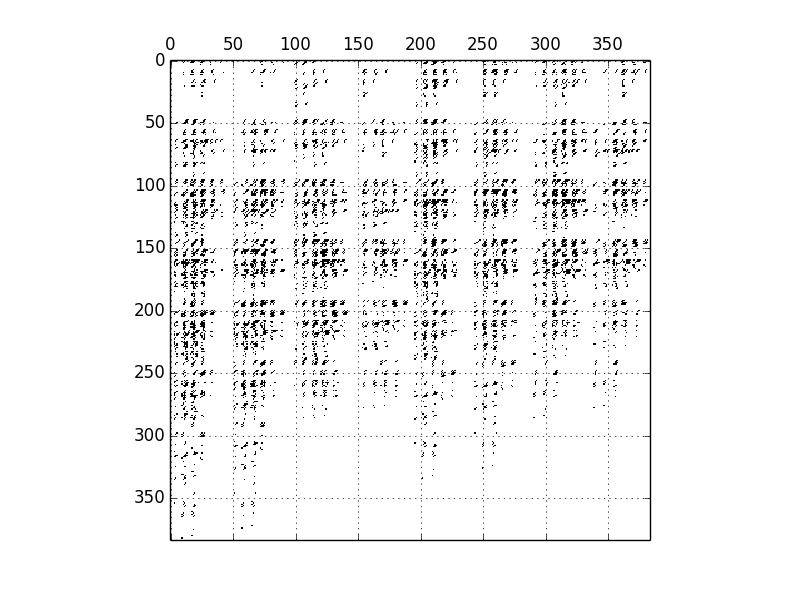
\includegraphics[width=8cm]{B0.png}
\end{center}

Ce système est de multidegré $(3, 2, 2, 2)$, la matrice de Bezout $B(1)$ est de taille $576$. Si on effectue une factorisation QRP sur cette matrice, on sait que les éléments diagonaux seront triés en ordre décroissant, voir figure ci-dessous.
\begin{center}
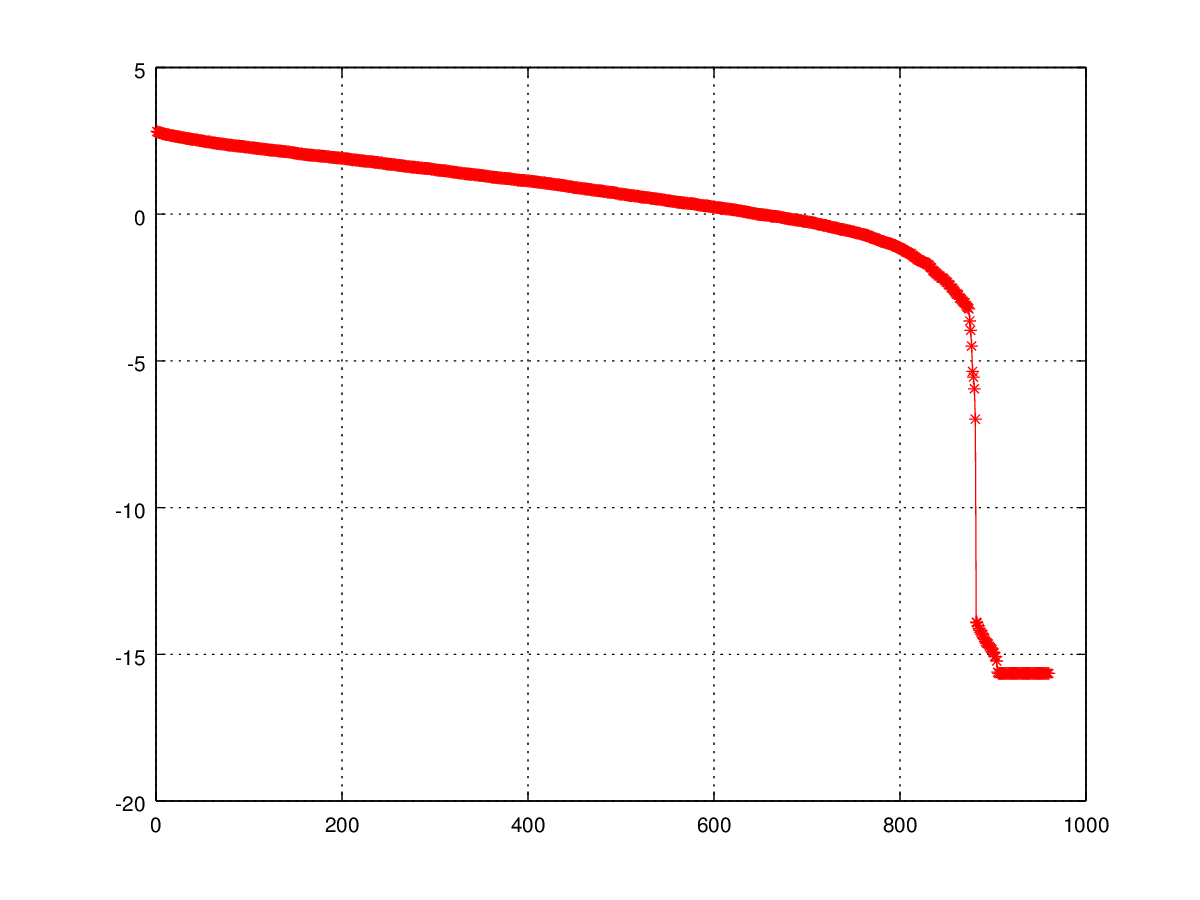
\includegraphics[width=8cm]{qrp.png}
\end{center}
 On s'aperçoit alors que les derniers éléments non nuls décroissent très vite, et qu'il peut devenir difficile de choisir un seuil au dessus duquel les éléments diagonaux seront déclarés ``non nuls''.
En d'autres termes, le ``saut'' entre éléments ``non-nuls'' et éléments proches du epsilon de la machine a tendance à diminuer à mesure que la taille de la matrice augmente, ce qui rend le calcul du rang numérique difficile.\\
Nous pouvons cependant améliorer un peu la situation précédente, en exploitant une propriété de $B(1)$. En effet, en permutant lignes et colones de cette matrice d'une certaine façon, on peut arriver à une structure bloc-triangulaire de $B(1)$.
\begin{center}
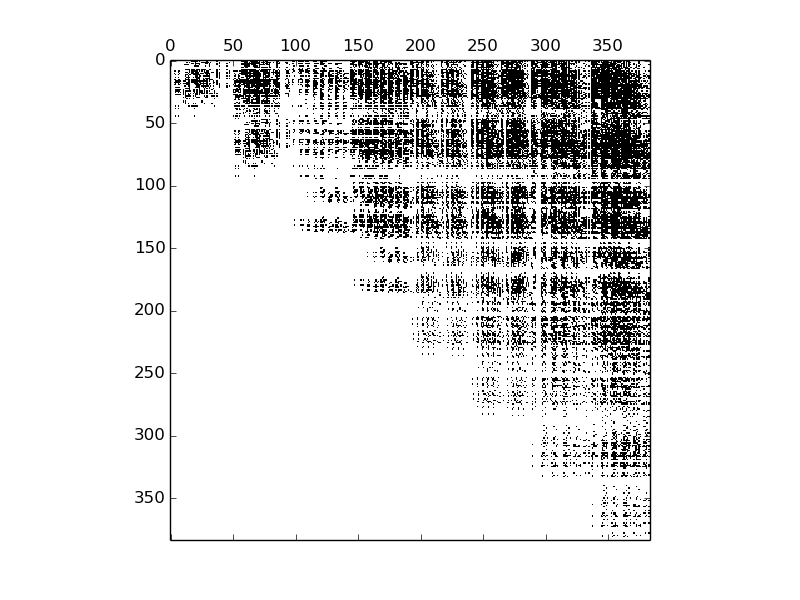
\includegraphics[width=8cm]{B0_tri.png}
\end{center}
En factorisant la matrice bloc après bloc, les éléments diagonaux vont alors décroitre uniquement à l'intérieur de chaque bloc, ce qui permet à la fin de préserver un saut numérique plus grand que dans la première approche. Le graphique ci dessous montre la nouvelle disposition des éléments diagonaux pour le même exemple que précédemment, traité de la deuxième façon.
\begin{center}
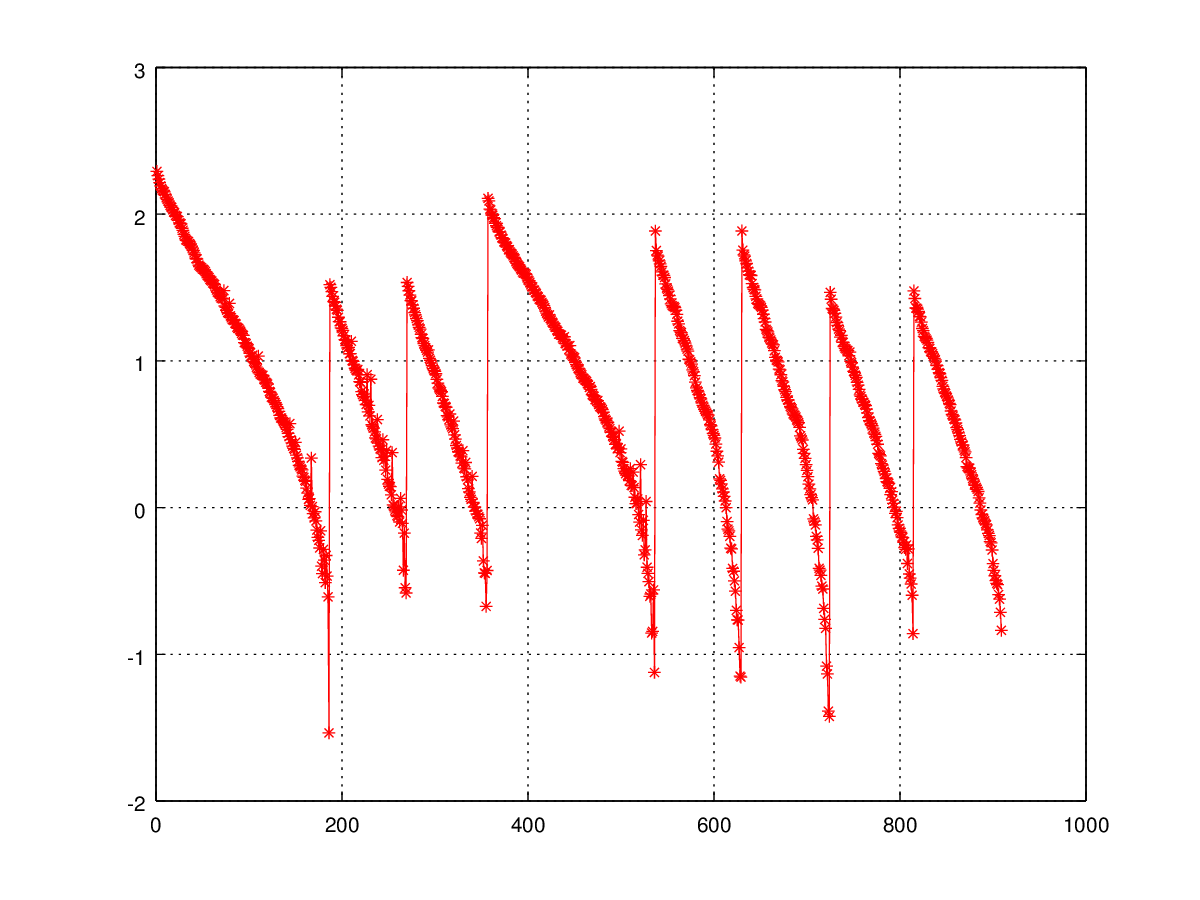
\includegraphics[width=8cm]{bloc_triang.png}
\end{center}
On voit que, malgré une décroissance rapide des éléments diagonaux dans chaque bloc, la plus petite taille de ceux-ci permet au plus petit élément ``non-nul" d'être beaucoup plus grand que le epsilon machine, ce qui facilite le calcul du rang numérique.

\end{document}
